\documentclass[border=8pt]{standalone}
\usepackage{tikz}
\usepackage{amsmath}
\usetikzlibrary{arrows.meta,calc,decorations.pathreplacing,positioning}

\begin{document}
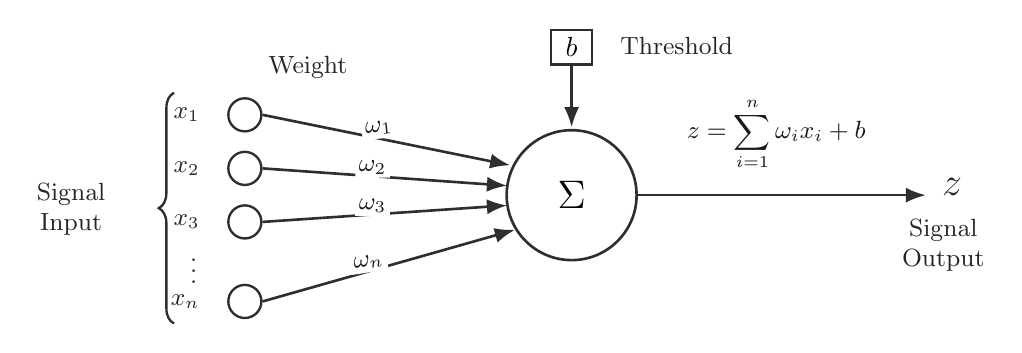
\begin{tikzpicture}[
  x=1cm,y=1cm,
  >=Latex,
  line/.style={draw=black!82,line width=0.85pt},
  arr/.style={-Latex,draw=black!82,line width=0.95pt},
  inputnode/.style={circle,draw=black!82,line width=0.85pt,minimum size=0.42cm,inner sep=0pt,fill=white},
  sumnode/.style={circle,draw=black!82,line width=0.95pt,minimum size=1.65cm,inner sep=0pt,fill=white},
  smallbox/.style={rectangle,draw=black!82,line width=0.85pt,minimum width=0.52cm,minimum height=0.44cm,inner sep=0pt,fill=white},
  textnode/.style={font=\small,black!85},
  lab/.style={font=\small,black!85,fill=white,inner sep=1.3pt},
  mathlab/.style={font=\small,black!90,fill=white,inner sep=1.3pt}
]

% ---------------- geometry, chosen to keep labels clear ----------------
\def\xSignal{-0.95}
\def\xBrace{-0.20}
\def\xInput{0.70}
\def\xSum{4.85}
\def\xOut{9.35}
\def\yOne{1.02}
\def\yTwo{0.34}
\def\yThree{-0.34}
\def\yN{-1.35}
\def\rSum{0.825}

% ---------------- signal input and input vector ----------------
\node[textnode,align=center,anchor=east] at (\xSignal,-0.18) {Signal\\Input};

\draw[line,decorate,decoration={brace,amplitude=5.5pt,mirror}]
  (\xBrace,\yOne+0.28) -- (\xBrace,\yN-0.28);

\node[textnode,anchor=east] at (\xInput-0.45,\yOne) {$x_1$};
\node[textnode,anchor=east] at (\xInput-0.45,\yTwo) {$x_2$};
\node[textnode,anchor=east] at (\xInput-0.45,\yThree) {$x_3$};
\node[textnode,anchor=east] at (\xInput-0.45,\yN) {$x_n$};
\node[textnode] at (\xInput-0.65,-0.86) {$\vdots$};

\node[inputnode] (x1) at (\xInput,\yOne) {};
\node[inputnode] (x2) at (\xInput,\yTwo) {};
\node[inputnode] (x3) at (\xInput,\yThree) {};
\node[inputnode] (xn) at (\xInput,\yN) {};

\node[textnode] at (\xInput+0.80,1.63) {Weight};

% ---------------- affine summation ----------------
\node[sumnode] (sum) at (\xSum,0) {\Large $\Sigma$};

% Arrow endpoints are explicit circle-boundary coordinates to avoid overlaps.
\coordinate (s1) at ($(sum.center)+(-0.78,0.38)$);
\coordinate (s2) at ($(sum.center)+(-0.82,0.12)$);
\coordinate (s3) at ($(sum.center)+(-0.82,-0.13)$);
\coordinate (sn) at ($(sum.center)+(-0.72,-0.44)$);

\draw[arr] (x1.east) -- (s1);
\draw[arr] (x2.east) -- (s2);
\draw[arr] (x3.east) -- (s3);
\draw[arr] (xn.east) -- (sn);

\node[mathlab,rotate=6]  at ($(x1.east)!0.47!(s1)+(0,0.13)$) {$\omega_1$};
\node[mathlab,rotate=1]  at ($(x2.east)!0.45!(s2)+(0,0.11)$) {$\omega_2$};
\node[mathlab,rotate=-1] at ($(x3.east)!0.45!(s3)+(0,0.11)$) {$\omega_3$};
\node[mathlab,rotate=9]  at ($(xn.east)!0.42!(sn)+(0,0.12)$) {$\omega_n$};

% ---------------- threshold ----------------
\node[smallbox] (b) at (\xSum,1.88) {$b$};
\node[textnode,anchor=west] at ($(b.east)+(0.22,0.02)$) {Threshold};
\draw[arr] (b.south) -- ($(sum.north)+(0,0.02)$);

% ---------------- affine output: no activation block ----------------
\draw[arr] (sum.east) -- (\xOut,0);

\node[mathlab,anchor=south] at ($(sum.east)!0.48!(\xOut,0)+(0,0.26)$)
  {$z=\displaystyle\sum_{i=1}^{n}\omega_i x_i+b$};

\node[textnode,anchor=west,font=\Large] at (\xOut+0.08,0.10) {$z$};
\node[textnode,align=center,anchor=north] at (\xOut+0.22,-0.18) {Signal\\Output};

\end{tikzpicture}
\end{document}
